% answers.tex —— 1987 年·上海卷·数学 · 参考答案与详细解析片段
% 由 tools/generate_projects.py 依来源总账自 1987/1987_数学真题_上海_试题.md + 1987/1987_数学真题_上海_解析正文.md + 1987/1987_数学真题_上海_答案要点.md 生成，勿手改（改源 MD 后重跑）


\begin{gktip}
固定源 PDF 无文字层，题面和答案与略解均依据高清页面读取。下列推导把固定源可见答案与必要的独立计算合并记录。
\end{gktip}

\begin{answer}
\gksolhead{1}{}

\textbf{题目}：

第一题（本题满分 36 分）共有 12 个小题，只要求直接填写结果，填对得 3 分，否则一律得 0 分。

（1） $y=x^3\ (x\leq0)$ 的反函数是 $\underline{\hspace{4em}}$。

\Needspace{5\baselineskip}
（2） 计算下式：

\nopagebreak[4]
\[
C_{10}^{1}+C_{10}^{2}+\cdots+C_{10}^{9}+C_{10}^{10}
\]

的值是 $\underline{\hspace{4em}}$。

\Needspace{5\baselineskip}
（3） 函数

\nopagebreak[4]
\[
f(x)=ax^2+bx+c
\]

是偶函数的充要条件是 $\underline{\hspace{4em}}$。

（4） 设 $ABCD-A_1B_1C_1D_1$ 为一正方体，$E,F$ 分别为 $BB_1,DC_1$ 的中点，则 $AE$ 与 $D_1F$ 所成的角为 $\underline{\hspace{4em}}$。

（5） 在底面半径为 $a$、高为 $2a$ 的圆柱中，分别挖去一个底面半径及高均为 $a$ 的圆锥与一个半径为 $a$ 的半球，则剩下部分的体积为 $\underline{\hspace{5em}}$。

\Needspace{5\baselineskip}
（6） 函数

\nopagebreak[4]
\[
y=2\left|\sin\left(4x-\frac\pi3\right)\right|
\]

的最小正周期为 $\underline{\hspace{4em}}$。

\Needspace{5\baselineskip}
（7） 计算函数值：

\nopagebreak[4]
\[
\arcsin\left(\sin\frac{3\pi}{5}\right)=\underline{\hspace{4em}}.
\]

\Needspace{5\baselineskip}
（8） 双曲线

\nopagebreak[4]
\[
4x^2-(y-3)^2=4
\]

的渐近线方程为 $\underline{\hspace{8em}}$。

\Needspace{5\baselineskip}
（9） 由参数方程

\nopagebreak[4]
\[
x=2(\sec^2\theta-1),\qquad y=2\operatorname{tg}\theta,
\qquad -\frac\pi2<\theta<\frac\pi2
\]

给出的曲线在直角坐标系下的方程为 $\underline{\hspace{6em}}$。

（10） 设 $\{a_n\}$ 为等差数列，已知 $a_1=1$，$a_5$ 与 $a_9$ 的算术平均数为 $19$，则该等差数列的公差为 $\underline{\hspace{4em}}$。

（11） $\left(x-\dfrac1x\right)^8$ 的展开式中，$x^4$ 的系数与 $\dfrac1{x^4}$ 的系数之差是 $\underline{\hspace{4em}}$。

\Needspace{5\baselineskip}
（12） 设 $2^a=5^b=10$，则

\nopagebreak[4]
\[
\frac1a+\frac1b=\underline{\hspace{4em}}.
\]

\Needspace{4\baselineskip}
\textbf{解析}

\gksubpart{（1）}

\Needspace{5\baselineskip}
由 $y=x^3$ 且 $x\le0$，交换变量可得反函数

\nopagebreak[4]
\[
y=-\sqrt[3]{x},\qquad x\le0.
\]

\gksubpart{（2）}

\Needspace{5\baselineskip}
利用二项式系数和

\nopagebreak[4]
\[
C_{10}^{1}+C_{10}^{2}+\cdots+C_{10}^{10}
=2^{10}-1=1023.
\]

\gksubpart{（3）}

\nopagebreak[4]
\[
f(-x)=ax^2-bx+c.
\]

对所有实数 $x$ 有 $f(-x)=f(x)$ 的充要条件是 $b=0$。

\gksubpart{（4）}

\Needspace{5\baselineskip}
建立单位正方体坐标。取

\nopagebreak[4]
\[
A=(0,0,0),\quad B=(1,0,0),\quad
D=(0,1,0),\quad A_1=(0,0,1),
\]

\Needspace{5\baselineskip}
则 $E$ 是 $BB_1$ 的中点，$F$ 是 $DC_1$ 的中点。可得

\nopagebreak[4]
\[
\overrightarrow{AE}\cdot\overrightarrow{D_1F}=0.
\]

所以两直线所成的角为 $\pi/2$。

\gksubpart{（5）}

\Needspace{5\baselineskip}
圆柱体积为 $2\pi a^3$。圆锥体积为 $\pi a^3/3$，半球体积为 $2\pi a^3/3$，故剩余体积为

\nopagebreak[4]
\[
2\pi a^3-\frac13\pi a^3-\frac23\pi a^3
=\pi a^3.
\]

\gksubpart{（6）}

\Needspace{5\baselineskip}
$|\sin u|$ 的最小正周期为 $\pi$。令 $u=4x-\pi/3$，得

\nopagebreak[4]
\[
4T=\pi,\qquad T=\frac\pi4.
\]

\gksubpart{（7）}

\nopagebreak[4]
\[
\sin\frac{3\pi}{5}=\sin\frac{2\pi}{5},
\]

\Needspace{5\baselineskip}
而反正弦函数的值域为 $[-\pi/2,\pi/2]$，所以

\nopagebreak[4]
\[
\arcsin\left(\sin\frac{3\pi}{5}\right)=\frac{2\pi}{5}.
\]

\gksubpart{（8）}

\Needspace{5\baselineskip}
由

\nopagebreak[4]
\[
4x^2-(y-3)^2=4
\]

\Needspace{5\baselineskip}
得渐近线

\nopagebreak[4]
\[
2x-(y-3)=0,\qquad 2x+(y-3)=0,
\]

即 $y=2x+3$ 和 $y=-2x+3$。

\gksubpart{（9）}

\Needspace{5\baselineskip}
由

\nopagebreak[4]
\[
x=2(\sec^2\theta-1)=2\operatorname{tg}^2\theta,
\qquad
y=2\operatorname{tg}\theta,
\]

\Needspace{5\baselineskip}
消去参数得

\nopagebreak[4]
\[
x=\frac{y^2}{2}.
\]

\gksubpart{（10）}

\Needspace{5\baselineskip}
等差数列中 $a_5$ 与 $a_9$ 的算术平均数等于 $a_7$，所以 $a_7=19$。由 $a_1=1$ 得

\nopagebreak[4]
\[
1+6d=19,\qquad d=3.
\]

\gksubpart{（11）}

\Needspace{5\baselineskip}
在

\nopagebreak[4]
\[
\left(x-\frac1x\right)^8
\]

\Needspace{5\baselineskip}
中，$x^4$ 项和 $x^{-4}$ 项分别对应二项式展开中的第 3 项和第 7 项，系数均为

\nopagebreak[4]
\[
\binom82=\binom86=28.
\]

两系数之差为 $0$。

\gksubpart{（12）}

\Needspace{5\baselineskip}
由 $2^a=5^b=10$，

\nopagebreak[4]
\[
\frac1a=\log_{10}2,\qquad
\frac1b=\log_{10}5.
\]

\Needspace{5\baselineskip}
所以

\nopagebreak[4]
\[
\frac1a+\frac1b=\log_{10}10=1.
\]

\gkanswer{答案（1）：$y=-\sqrt[3]{x}\ (x\leq0)$}

\gkanswer{答案（2）：$1023$}

\gkanswer{答案（3）：$b=0$}

\gkanswer{答案（4）：$\dfrac\pi2$}

\gkanswer{答案（5）：$\pi a^3$}

\gkanswer{答案（6）：$\dfrac\pi4$}

\gkanswer{答案（7）：$\dfrac{2\pi}{5}$}

\gkanswer{答案（8）：$y=2x+3,\ y=-2x+3$}

\gkanswer{答案（9）：$x=\dfrac{y^2}{2}$}

\gkanswer{答案（10）：$3$}

\gkanswer{答案（11）：$0$}

\gkanswer{答案（12）：$1$}

\end{answer}
\begin{answer}
\gksolhead{2}{}

\textbf{题目}：

第二题（本题满分 36 分）共有 12 个小题，每题都给出代号为 A、B、C、D 的四个结论，其中有一个结论是正确的；选对得 3 分，不选、选错或选出的代号超过一个，一律得 0 分。

\Needspace{5\baselineskip}
（1） 设函数

\nopagebreak[4]
\[
y=\log_2x+3\qquad(x\geq1),
\]

则 $y$ 的值域是\mbox{（　　）}

（A）$\{y\mid y\geq3\}$　　（B）$\{y\mid y>3\}$

（C）$\{y\mid y\geq5\}$　　（D）$R$

（2） 下列函数图象中，表示 $y=x^{\frac23}$ 的是\mbox{（　　）}
\nopagebreak[4]
\begin{center}% 1987 年上海卷第二题：y=x^(2/3) 的四个图象选项
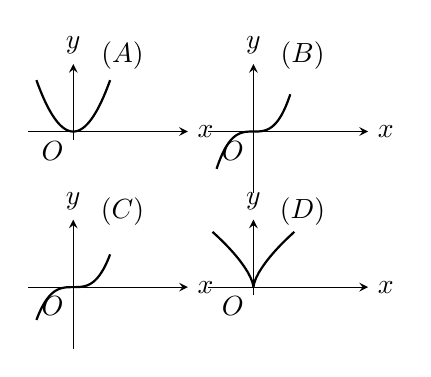
\begin{tikzpicture}[scale=0.52,>=stealth]
  \node at (1.2,1.85) {$(A)$};
  \draw[->] (-1.1,0)--(2.8,0) node[right] {$x$};
  \draw[->] (0,-0.2)--(0,1.65) node[above] {$y$};
  \draw[thick,domain=-0.9:0.9,samples=80] plot (\x,{1.55*\x*\x});
  \node[below left] at (0,0) {$O$};

  \begin{scope}[xshift=4.4cm]
    \node at (1.2,1.85) {$(B)$};
    \draw[->] (-1.1,0)--(2.8,0) node[right] {$x$};
    \draw[->] (0,-1.5)--(0,1.65) node[above] {$y$};
    \draw[thick,domain=-0.9:0.9,samples=80] plot (\x,{1.25*\x*\x*\x});
    \node[below left] at (0,0) {$O$};
  \end{scope}

  \begin{scope}[yshift=-3.8cm]
    \node at (1.2,1.85) {$(C)$};
    \draw[->] (-1.1,0)--(2.8,0) node[right] {$x$};
    \draw[->] (0,-1.5)--(0,1.65) node[above] {$y$};
    \draw[thick,domain=-0.9:0.9,samples=80] plot (\x,{1.1*\x*\x*\x});
    \node[below left] at (0,0) {$O$};
  \end{scope}

  \begin{scope}[xshift=4.4cm,yshift=-3.8cm]
    \node at (1.2,1.85) {$(D)$};
    \draw[->] (-1.1,0)--(2.8,0) node[right] {$x$};
    \draw[->] (0,-0.2)--(0,1.65) node[above] {$y$};
    \draw[thick,domain=-1.0:0,samples=80] plot (\x,{1.35*abs(\x)^(2/3)});
    \draw[thick,domain=0:1.0,samples=80] plot (\x,{1.35*abs(\x)^(2/3)});
    \node[below left] at (0,0) {$O$};
  \end{scope}
\end{tikzpicture}
\end{center}
\nopagebreak[4]
（3） 设实数 $a,b$ 满足 $0<a<b$ 且 $a+b=1$，则下列四数中最大的是\mbox{（　　）}

（A）$\dfrac12$　　（B）$a^2+b^2$　　（C）$2ab$　　（D）$a$

（4） 设 $0<\theta<45^\circ$，则 $\cos^2\theta,\sin^2\theta,\operatorname{ctg}^2\theta$ 的大小规律是\mbox{（　　）}

（A）$\cos^2\theta<\sin^2\theta<\operatorname{ctg}^2\theta$

（B）$\operatorname{ctg}^2\theta<\sin^2\theta<\cos^2\theta$

（C）$\sin^2\theta<\cos^2\theta<\operatorname{ctg}^2\theta$

（D）$\cos^2\theta<\operatorname{ctg}^2\theta<\sin^2\theta$

\Needspace{5\baselineskip}
（5） 计算下式：

\nopagebreak[4]
\[
\frac{\sin\alpha+\sin\beta}{\cos\alpha+\cos\beta}
\]

等于\mbox{（　　）}

（A）$\operatorname{tg}\dfrac{\alpha+\beta}{2}$　　（B）$-\operatorname{tg}\dfrac{\alpha+\beta}{2}$

（C）$\operatorname{tg}\alpha+\operatorname{tg}\beta$　　（D）$\operatorname{ctg}\dfrac{\alpha+\beta}{2}$

\Needspace{5\baselineskip}
（6） 如果圆

\nopagebreak[4]
\[
x^2+y^2+ax+by+c=0\qquad(a,b,c\text{ \text{不全为} }0)
\]

与 $x$ 轴相切于原点，那么\mbox{（　　）}

（A）$a=0,\ b\ne0,\ c\ne0$　　（B）$b=c=0,\ a\ne0$

（C）$a=c=0,\ b\ne0$　　（D）$a=b=0,\ c\ne0$

（7） 直线 $x+2y+3=0$ 的倾斜角为\mbox{（　　）}

（A）$\operatorname{arctg}\left(-\dfrac12\right)$　　（B）$\operatorname{arctg}\dfrac12$

（C）$\dfrac\pi2+\operatorname{arctg}\dfrac12$　　（D）$\pi-\operatorname{arctg}\dfrac12$

\Needspace{5\baselineskip}
（8） 极坐标方程

\nopagebreak[4]
\[
\rho=\frac6{3+2\sin\left(\frac32\pi+\theta\right)}
\]

所表示的图形是\mbox{（　　）}

（A）圆　　（B）椭圆　　（C）双曲线　　（D）抛物线

（9） 在空间里，下述命题中正确的是\mbox{（　　）}

（A）若直线 $a\parallel$ 平面 $M$，直线 $b\perp$ 直线 $a$，则直线 $b\perp$ 平面 $M$。

（B）若平面 $M\parallel$ 平面 $N$，则平面 $M$ 内任意一条直线 $a\parallel$ 平面 $N$。

（C）若平面 $M$ 与平面 $N$ 的交线为 $a$，平面 $M$ 内的直线 $b\perp$ 直线 $a$，则直线 $b\perp$ 平面 $N$。

（D）若平面 $N$ 内的两条直线都平行于平面 $M$，则平面 $N\parallel$ 平面 $M$。

（10） 三个互不重合的平面能把空间分成 $n$ 个部分，$n$ 的所有可能值为\mbox{（　　）}

（A）$4,6,7$　　（B）$4,5,6,8$　　（C）$4,7,8$　　（D）$4,6,7,8$

\Needspace{5\baselineskip}
（11） 若直线

\nopagebreak[4]
\[
l_1:ax+2y+6=0
\]

\Needspace{5\baselineskip}
与直线

\nopagebreak[4]
\[
l_2:x+(a-1)y+(a^2-1)=0
\]

平行但不重合，则 $a$ 等于\mbox{（　　）}

（A）$-1$ 或 $2$　　（B）$-1$　　（C）$2$　　（D）$\dfrac23$

（12） 七人并排成一行，如果甲、乙两人必须不相邻，那么不同排法的种数是\mbox{（　　）}

（A）1440　　（B）3600　　（C）4320　　（D）4800

\Needspace{4\baselineskip}
\textbf{解析}

\gksubpart{（1）}

因为 $x\ge1$，$\log_2x\ge0$，且能取遍 $[0,+\infty)$，故值域为 $[3,+\infty)$，答案为 A。

\gksubpart{（2）}

$y=x^{2/3}$ 的定义域为全体实数，值域为非负数，且关于 $y$ 轴对称，在原点处有尖点。因此对应固定源图形中的 D。

\gksubpart{（3）}

\Needspace{5\baselineskip}
由 $a+b=1$ 和 $0<a<b$，有 $0<a<1/2$。于是

\nopagebreak[4]
\[
a^2+b^2-\frac12=\frac12(a-b)^2>0,
\]

\Needspace{5\baselineskip}
且

\nopagebreak[4]
\[
a^2+b^2-a=(2a-1)(a-1)>0.
\]

同时 $2ab<1/2$，所以最大者为 $a^2+b^2$，答案为 B。

\gksubpart{（4）}

\Needspace{5\baselineskip}
当 $0<\theta<45^\circ$ 时，

\nopagebreak[4]
\[
0<\sin^2\theta<\cos^2\theta<1
\]

\Needspace{5\baselineskip}
且 $\operatorname{ctg}^2\theta>1$。故

\nopagebreak[4]
\[
\sin^2\theta<\cos^2\theta<\operatorname{ctg}^2\theta,
\]

答案为 A。

\gksubpart{（5）}

\Needspace{5\baselineskip}
和差化积得

\nopagebreak[4]
\[
\frac{\sin\alpha+\sin\beta}{\cos\alpha+\cos\beta}
=\frac{2\sin\frac{\alpha+\beta}{2}\cos\frac{\alpha-\beta}{2}}
{2\cos\frac{\alpha+\beta}{2}\cos\frac{\alpha-\beta}{2}}
=\operatorname{tg}\frac{\alpha+\beta}{2}.
\]

答案为 A。

\gksubpart{（6）}

\Needspace{5\baselineskip}
圆与 $x$ 轴相切于原点，首先必须过原点，所以 $c=0$。在原点处圆的切线为

\nopagebreak[4]
\[
ax+by=0
\]

的切线方向；要使其为 $x$ 轴，需 $a=0$ 且 $b\ne0$。故答案为 C。

\gksubpart{（7）}

\Needspace{5\baselineskip}
直线斜率为 $-1/2$，其倾斜角属于第二象限，因此

\nopagebreak[4]
\[
\alpha=\pi-\arctan\frac12
=\frac\pi2+\arctan\frac12.
\]

答案为 C。

\gksubpart{（8）}

\Needspace{5\baselineskip}
因为 $\sin(3\pi/2+\theta)=-\cos\theta$，原式化为

\nopagebreak[4]
\[
\rho=\frac6{3-2\cos\theta}.
\]

\Needspace{5\baselineskip}
于是

\nopagebreak[4]
\[
3\rho=6+2x.
\]

\Needspace{5\baselineskip}
平方并整理得

\nopagebreak[4]
\[
5x^2+9y^2-24x-36=0,
\]

这是椭圆，答案为 B。

\gksubpart{（9）}

选项 B 由平行平面的性质直接成立：若 $M\parallel N$，则 $M$ 内任意直线均不与 $N$ 相交，因而平行于 $N$。其余选项缺少必要的垂直或相交条件，答案为 B。

\gksubpart{（10）}

三个平面可取为全平行、两个平行而第三个相交、三条交线平行或三平面一般位置，分别得到 $4,6,7,8$ 个区域。答案为 D。

\gksubpart{（11）}

\Needspace{5\baselineskip}
两直线平行要求

\nopagebreak[4]
\[
a(a-1)=2,
\]

\Needspace{5\baselineskip}
所以 $a=2$ 或 $a=-1$。当 $a=2$ 时两方程互为倍数而重合，故只能取

\nopagebreak[4]
\[
a=-1.
\]

答案为 B。

\gksubpart{（12）}

\Needspace{5\baselineskip}
七人全排列有 $7!=5040$ 种。甲乙相邻时，把二人看作一个整体并计入内部两种顺序，有

\nopagebreak[4]
\[
2\cdot6!=1440
\]

\Needspace{5\baselineskip}
种。因此不相邻的排法为

\nopagebreak[4]
\[
7!-2\cdot6!=3600.
\]

答案为 B。

\gkanswer{答案（1）：A}

\gkanswer{答案（2）：D}

\gkanswer{答案（3）：B}

\gkanswer{答案（4）：A}

\gkanswer{答案（5）：A}

\gkanswer{答案（6）：C}

\gkanswer{答案（7）：C}

\gkanswer{答案（8）：B}

\gkanswer{答案（9）：B}

\gkanswer{答案（10）：D}

\gkanswer{答案（11）：B}

\gkanswer{答案（12）：B}

\end{answer}
\begin{answer}
\gksolhead{3}{}

\textbf{题目}：

\Needspace{5\baselineskip}
第三题（本题满分 7 分）。设

\nopagebreak[4]
\[
A=\left\{x\middle|\log_{\frac13}\left|x-\frac\pi3\right|
\geq\log_{\frac13}\frac{2\pi}{3},\ x\in R\right\},
\]

\nopagebreak[4]
\[
B=\{x\mid\cos x\geq0,\ x\in R\}.
\]

求 $D=A\cap B$，最后结果用区间形式表示，并在数轴上标出符合 $D$ 的部分。

\Needspace{4\baselineskip}
\textbf{解析}

\Needspace{5\baselineskip}
由底数 $1/3<1$，不等式方向反转：

\nopagebreak[4]
\[
\left|x-\frac\pi3\right|\le\frac{2\pi}{3}.
\]

\Needspace{5\baselineskip}
故

\nopagebreak[4]
\[
A=\left[-\frac\pi3,\pi\right].
\]

\Needspace{5\baselineskip}
又

\nopagebreak[4]
\[
B=\{x\mid\cos x\ge0\}.
\]

\Needspace{5\baselineskip}
在 $A$ 的范围内，只有区间 $\left[-\pi/3,\pi/2\right]$ 满足 $\cos x\ge0$，所以

\nopagebreak[4]
\[
D=A\cap B=\left[-\frac\pi3,\frac\pi2\right].
\]

\gkanswer{答案：$\displaystyle D=\left[-\frac\pi3,\frac\pi2\right]$}

\end{answer}
\begin{answer}
\gksolhead{4}{}

\textbf{题目}：

\Needspace{5\baselineskip}
第四题（本题满分 8 分）共有 3 个小题。设三棱锥 $S-ABC$ 的底面为等腰直角三角形，已知该直角三角形的斜边 $AC$ 长为 $10$，三棱锥的侧棱

\nopagebreak[4]
\[
SA=SB=SC=13.
\]

（1） 顶点 $S$ 到底面的距离；

（2） 侧棱 $SB$ 与底面所成角的大小（用反三角函数表示）；

（3） 二面角 $A-SB-C$ 的大小（用反三角函数表示）。
\nopagebreak[4]
\begin{center}% 1987 年上海卷第四题：三棱锥 S-ABC
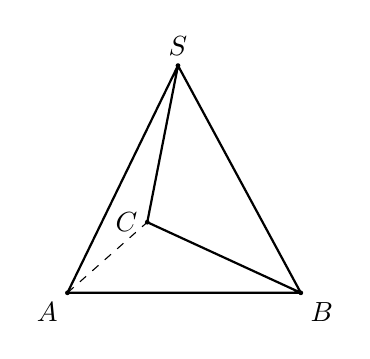
\begin{tikzpicture}[scale=0.78,>=stealth]
  \coordinate (S) at (1.8,3.7);
  \coordinate (A) at (0,0);
  \coordinate (B) at (3.8,0);
  \coordinate (C) at (1.3,1.15);
  \draw[thick] (S)--(A) (S)--(B) (S)--(C) (A)--(B) (B)--(C);
  \draw[dashed] (A)--(C);
  \fill (S) circle (1.1pt) node[above] {$S$};
  \fill (A) circle (1.1pt) node[below left] {$A$};
  \fill (B) circle (1.1pt) node[below right] {$B$};
  \fill (C) circle (1.1pt) node[left] {$C$};
\end{tikzpicture}
\end{center}
\nopagebreak[4]
\Needspace{4\baselineskip}
\textbf{解析}

\gksubpart{（1）}

\Needspace{5\baselineskip}
设底面直角等腰三角形的直角顶点为 $B$，则 $AC=10$ 为斜边，底面外接圆圆心 $O$ 是 $AC$ 的中点，故

\nopagebreak[4]
\[
OA=OB=OC=5.
\]

\Needspace{5\baselineskip}
因 $SA=SB=SC$，顶点 $S$ 在过 $O$ 的底面垂线上。于是

\nopagebreak[4]
\[
SO=\sqrt{SA^2-OA^2}
=\sqrt{13^2-5^2}=12.
\]

\gksubpart{（2）}

\Needspace{5\baselineskip}
侧棱 $SB$ 在底面上的射影为 $BO=5$，所以侧棱与底面所成角 $\alpha$ 满足

\nopagebreak[4]
\[
\sin\alpha=\frac{SO}{SB}=\frac{12}{13},
\]

\Needspace{5\baselineskip}
即

\nopagebreak[4]
\[
\alpha=\arcsin\frac{12}{13}.
\]

\gksubpart{（3）}

\Needspace{5\baselineskip}
取坐标

\nopagebreak[4]
\[
A=(-5,0,0),\quad C=(5,0,0),\quad B=(0,5,0),\quad S=(0,0,12).
\]

\Needspace{5\baselineskip}
两侧面的法向量可取

\nopagebreak[4]
\[
n_1=(60,-60,-25),\qquad n_2=(60,60,25).
\]

\Needspace{5\baselineskip}
两平面的锐角 $\varphi$ 满足

\nopagebreak[4]
\[
\cos\varphi=\frac{25}{313},\qquad
\sin\varphi=\frac{312}{313}.
\]

\Needspace{5\baselineskip}
因此

\nopagebreak[4]
\[
\tan\frac\varphi2
=\frac{\sin\varphi}{1+\cos\varphi}
=\frac{12}{13},
\]

\Needspace{5\baselineskip}
从而二面角为

\nopagebreak[4]
\[
\varphi=2\arctan\frac{12}{13}.
\]

\gkanswer{答案（1）：$SO=12$}

\gkanswer{答案（2）：$\displaystyle\arcsin\frac{12}{13}$}

\gkanswer{答案（3）：$\displaystyle2\arctan\frac{12}{13}$}

\end{answer}
\begin{answer}
\gksolhead{5}{}

\textbf{题目}：

\Needspace{5\baselineskip}
第五题（本题满分 9 分）。设 $A(x_1,y_1)$ 为椭圆

\nopagebreak[4]
\[
x^2+2y^2=2
\]

\Needspace{5\baselineskip}
上的任意一点，过点 $A$ 作一条斜率为

\nopagebreak[4]
\[
-\frac{x_1}{2y_1}
\]

\Needspace{5\baselineskip}
的直线 $l$，又设 $d$ 为原点到直线 $l$ 的距离，$r_1,r_2$ 分别为点 $A$ 到椭圆两个焦点的距离。试证明

\nopagebreak[4]
\[
\sqrt{r_1r_2}\cdot d
\]

为常数。

\Needspace{4\baselineskip}
\textbf{解析}

\Needspace{5\baselineskip}
椭圆

\nopagebreak[4]
\[
x^2+2y^2=2
\]

\Needspace{5\baselineskip}
的两个焦点为 $F_1(-1,0),F_2(1,0)$。对点 $A(x_1,y_1)$，

\nopagebreak[4]
\[
r_1^2=(x_1+1)^2+y_1^2,\qquad
r_2^2=(x_1-1)^2+y_1^2.
\]

\Needspace{5\baselineskip}
利用 $x_1^2+2y_1^2=2$，可得

\nopagebreak[4]
\[
r_1^2r_2^2=(1+y_1^2)^2,
\qquad
r_1r_2=1+y_1^2.
\]

\Needspace{5\baselineskip}
过 $A$ 且斜率为 $-x_1/(2y_1)$ 的直线为

\nopagebreak[4]
\[
x_1x+2y_1y=2.
\]

\Needspace{5\baselineskip}
故原点到该直线的距离为

\nopagebreak[4]
\[
d=\frac2{\sqrt{x_1^2+4y_1^2}}
=\frac{\sqrt2}{\sqrt{1+y_1^2}}.
\]

\Needspace{5\baselineskip}
于是

\nopagebreak[4]
\[
\sqrt{r_1r_2}\,d
=\sqrt{1+y_1^2}\cdot
\frac{\sqrt2}{\sqrt{1+y_1^2}}
=\sqrt2,
\]

确为常数。

\gkanswer{答案：$\displaystyle\sqrt{r_1r_2}\,d=\sqrt2$}

\end{answer}
\begin{answer}
\gksolhead{6}{}

\textbf{题目}：

第六题（本题满分 12 分）本题共有 2 个小题，第 1 小题满分 5 分，第 2 小题满分 7 分。

\Needspace{5\baselineskip}
在 $xOy$ 平面上给定一曲线

\nopagebreak[4]
\[
y^2=2x.
\]

（1） 设点 $A$ 的坐标为 $\left(\frac23,0\right)$，求曲线上距点 $A$ 最近的点 $P$ 之坐标及相应的距离 $|PA|$；

（2） 设点 $A$ 的坐标为 $(a,0)$，$a\in R$，求曲线上点距点 $A$ 的距离之最小值，并写出 $d=f(a)$ 的函数表达式。

\Needspace{4\baselineskip}
\textbf{解析}

\Needspace{5\baselineskip}
曲线为 $y^2=2x$，点 $A=(a,0)$。曲线上点 $P=(x,y)$ 的距离平方为

\nopagebreak[4]
\[
|PA|^2=(x-a)^2+y^2
=(x-a)^2+2x
=\left(x-a+1\right)^2+2a-1,
\qquad x\ge0.
\]

\gksubpart{（1）}

\Needspace{5\baselineskip}
当 $a=2/3<1$ 时，右端在 $x=0$ 处取得最小值。因此

\nopagebreak[4]
\[
P=(0,0),\qquad |PA|=\frac23.
\]

\gksubpart{（2）}

\Needspace{5\baselineskip}
当 $a\ge1$ 时，最小点的横坐标为 $x=a-1$，最小距离为 $\sqrt{2a-1}$；当 $a<1$ 时，边界 $x=0$ 取得最小值，最小距离为 $|a|$。所以

\nopagebreak[4]
\[
d=f(a)=
\begin{cases}
\sqrt{2a-1},&a\ge1,\\
|a|,&a<1.
\end{cases}
\]

\gkanswer{答案（1）：$P=(0,0)$，$|PA|=\dfrac23$}

\gkanswer{答案（2）：见解析版}

\end{answer}
\begin{answer}
\gksolhead{7}{}

\textbf{题目}：

第七题（本题满分 12 分）本题共有 3 个小题，第 1 小题满分 4 分，第 2 小题满分 5 分，第 3 小题满分 3 分。

设复平面上有一系列向量 $\overrightarrow{OZ_n}$（$n=0,1,2,\ldots$）满足如下关系：将 $\overrightarrow{OZ_n}$ 逆时针方向旋转 $\frac34\pi$ 后，再把它的模变为原来的一半，得到 $\overrightarrow{OZ_{n+1}}$。记 $\overrightarrow{OZ_n}$ 所对应的复数为 $z_n$（$n=0,1,2,\ldots$）。

\Needspace{5\baselineskip}
若

\nopagebreak[4]
\[
z_0=2\sqrt2+2\sqrt2\,i,
\]

且复数的辐角为辐角的主值，

（1） 求 $z_n$；

（2） $n$ 为何值时，$z_n$ 为实数？将所有等于实数的 $z_n$ 按原有次序排成数列 $\{a_n\}$，写出该数列的通项公式；

\Needspace{5\baselineskip}
（3） 求

\nopagebreak[4]
\[
\lim_{k\to\infty}(a_1+a_2+\cdots+a_k).
\]

\Needspace{4\baselineskip}
\textbf{解析}

\Needspace{5\baselineskip}
每次旋转并缩短对应的复数乘以

\nopagebreak[4]
\[
q=\frac12\left(\cos\frac{3\pi}{4}
+i\sin\frac{3\pi}{4}\right)
=\frac{-1+i}{2\sqrt2}.
\]

\gksubpart{（1）}

\Needspace{5\baselineskip}
由 $z_0=2\sqrt2+2\sqrt2\,i=2\sqrt2(1+i)$，得

\nopagebreak[4]
\[
z_n=2\sqrt2(1+i)
\left(\frac{-1+i}{2\sqrt2}\right)^n.
\]

\gksubpart{（2）}

\Needspace{5\baselineskip}
$z_0$ 的辐角为 $\pi/4$，所以 $z_n$ 的辐角为

\nopagebreak[4]
\[
\frac\pi4+\frac{3n\pi}{4}.
\]

\Needspace{5\baselineskip}
它为实数当且仅当该角是 $\pi$ 的整数倍，即

\nopagebreak[4]
\[
n=4k+1,\qquad k=0,1,2,\ldots.
\]

\Needspace{5\baselineskip}
并且 $q^4=-1/16$、$z_1=-2$，故按原次序排列的实数项为

\nopagebreak[4]
\[
a_k=-2\left(-\frac1{16}\right)^{k-1},
\qquad k=1,2,\ldots.
\]

\gksubpart{（3）}

\Needspace{5\baselineskip}
这是首项 $-2$、公比 $-1/16$ 的等比级数，因此

\nopagebreak[4]
\[
\lim_{k\to\infty}(a_1+\cdots+a_k)
=\frac{-2}{1-(-1/16)}
=-\frac{32}{17}.
\]

\gkanswer{答案（1）：$\displaystyle z_n=2\sqrt2(1+i)\left(\frac{-1+i}{2\sqrt2}\right)^n$}

\gkanswer{答案（2）：$n=4k+1\ (k=0,1,2,\ldots)$；$\displaystyle a_k=-2\left(-\frac1{16}\right)^{k-1}$}

\gkanswer{答案（3）：$\displaystyle-\frac{32}{17}$}

\end{answer}